\section{Recurrent Neural Networks (RNN)}
\begin{frame}{}
    \LARGE Advanced Computer Vision: \textbf{Recurrent Neural Networks (RNN)}
\end{frame}

\begin{frame}[allowframebreaks]{Recurrent Neural Networks (RNN)}
    \textbf{What are RNNs?}
        \begin{itemize}
            \item Neural networks designed for sequence data.
            \item Maintain a hidden state $h_t$ that carries information from previous time steps.
            \item Recurrent architecture: $h_t = f(h_{t-1}, x_t)$
        \end{itemize}
    \vspace{0.5cm}
    \textbf{Use Cases:}
        \begin{itemize}
            \item Language modeling
            \item Time series prediction
            \item Sequence classification
        \end{itemize}
    
\framebreak

    \begin{columns}
        \begin{column}{0.4\textwidth}
            \begin{figure}
            \centering
            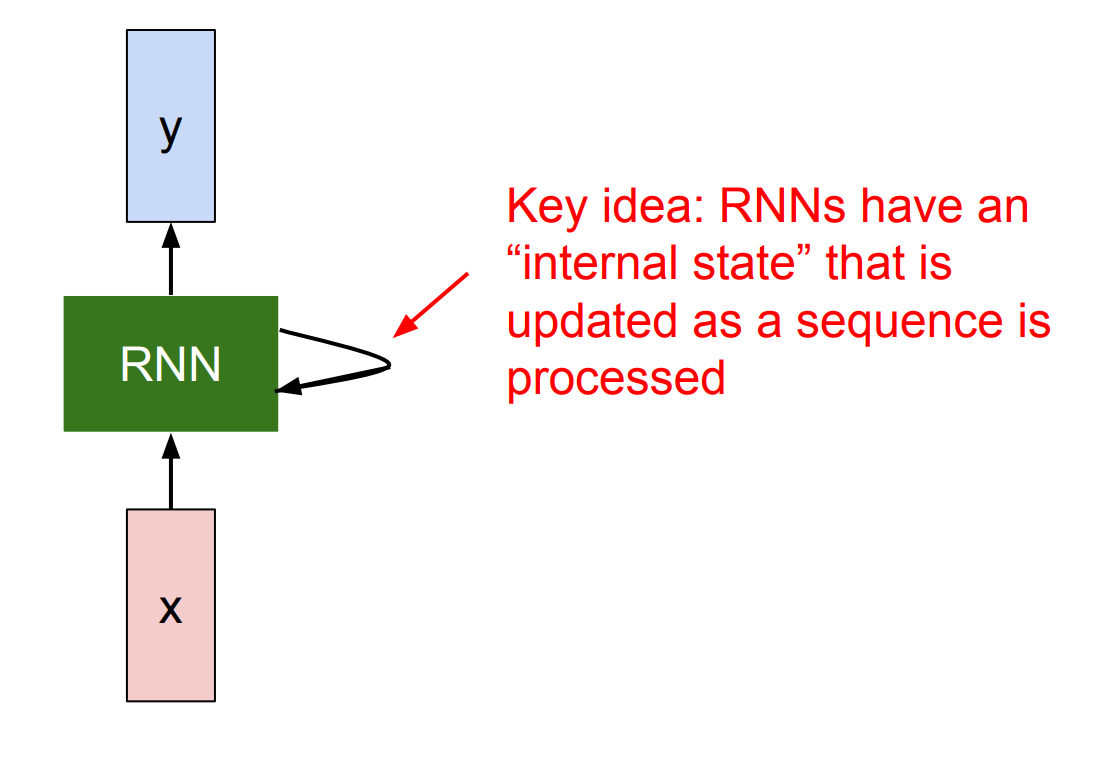
\includegraphics[width=1.0\textwidth,height=1.0\textheight,keepaspectratio]{images/advanced-cv/rnn_1.png}
            \end{figure}
        \end{column}
        \begin{column}{0.6\textwidth}
            \begin{figure}
            \centering
            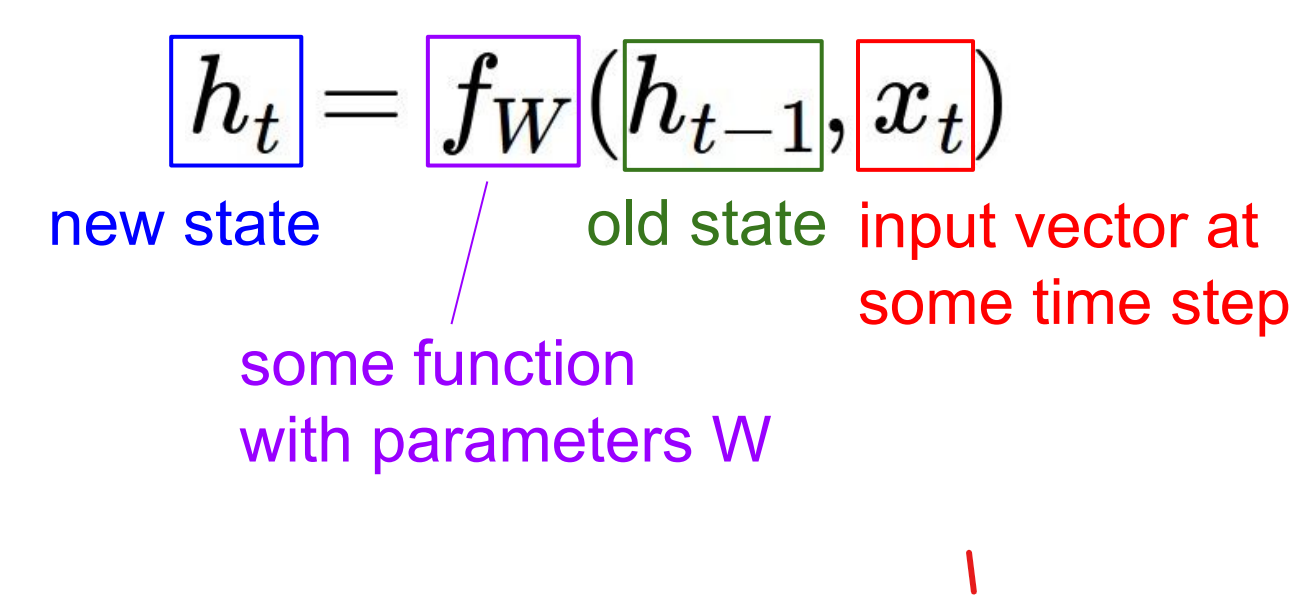
\includegraphics[width=1.0\textwidth,height=1.0\textheight,keepaspectratio]{images/advanced-cv/rnn_2.png}
            \end{figure}        
        \end{column}
    \end{columns}

\framebreak

    \begin{figure}
    \centering
    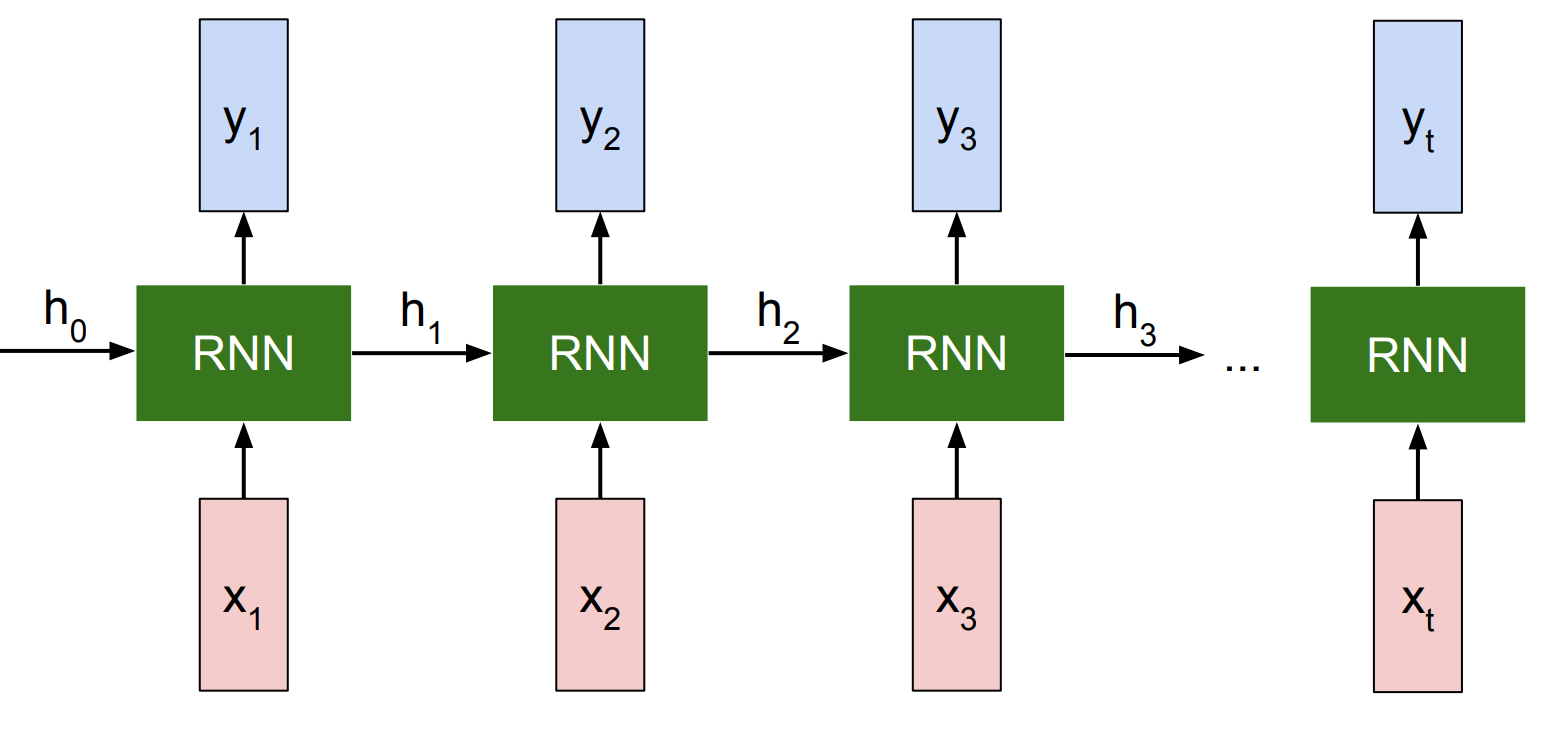
\includegraphics[width=1.0\textwidth,height=1.0\textheight,keepaspectratio]{images/advanced-cv/rnn_3.png}
    \end{figure}  

\framebreak

    \begin{figure}
    \centering
    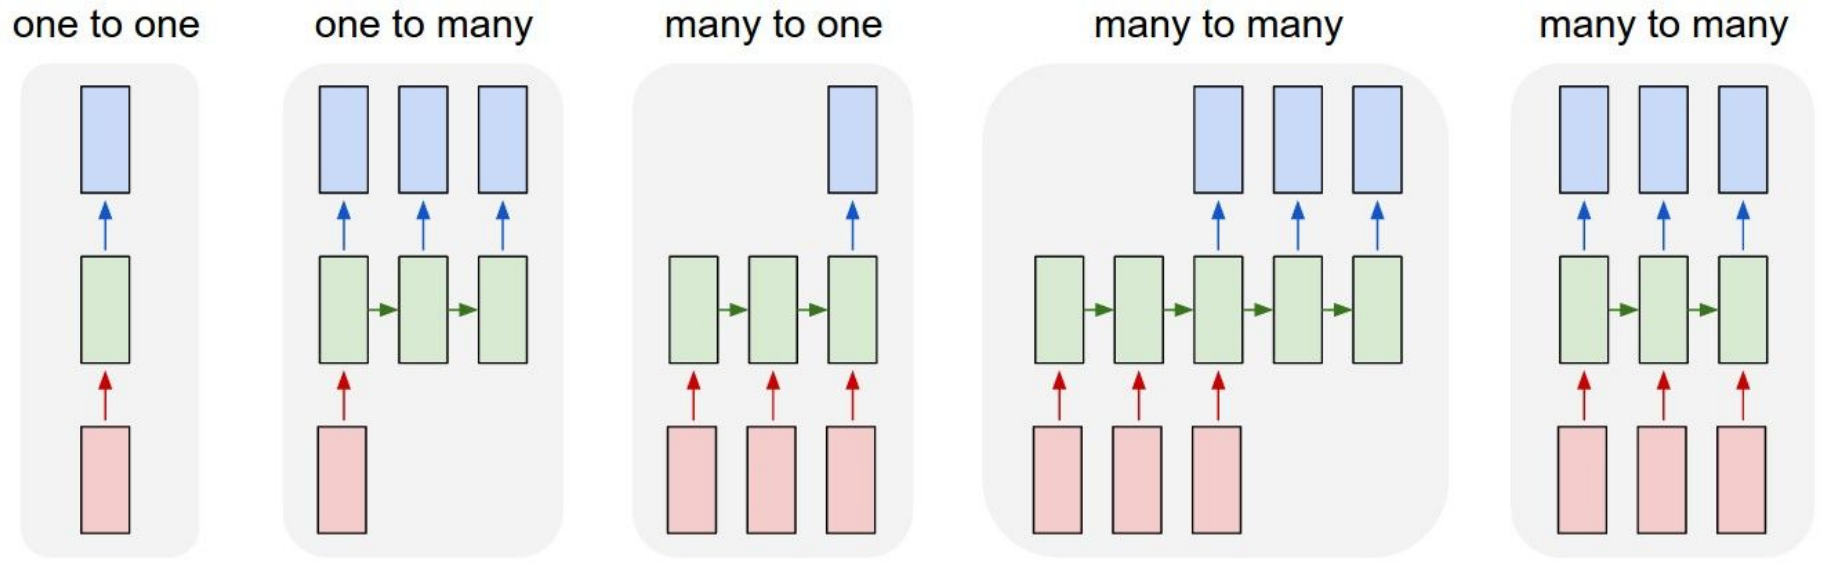
\includegraphics[width=1.0\textwidth,height=1.0\textheight,keepaspectratio]{images/advanced-cv/rnn_4.png}
    \end{figure}  

\framebreak
    
    \large RNN Advantages:
        \begin{itemize}
            \item Can process any length input
            \item Computation for step t can (in theory) use information from many steps back 
            \item Model size doesn’t increase for longer input 
            \item Same weights applied on every timestep, so there is symmetry in how inputs are processed. 
        \end{itemize}

\framebreak

    \large RNN Disadvantages:
        \begin{itemize}
            \item Recurrent computation is slow 
            \item In practice, difficult to access information from many steps back
        \end{itemize}
    \vspace{0.5cm}
    \large Limitations of RNNs:
        \begin{itemize}
            \item Vanishing/exploding gradients in long sequences.
            \item Sequential computation --- slow to train.
            \item Difficulty in capturing long-term dependencies.
            \item Cannot parallelize easily due to recursive nature.
        \end{itemize}
\end{frame}
